
\documentclass{beamer}

\usetheme{default}
\usecolortheme{beaver}

\usepackage[german]{babel}
\usepackage[utf8]{inputenc}

\usepackage[sfdefault]{roboto}
\usepackage{textcomp}

\usepackage{graphicx}
\graphicspath{{./images/}}

\usepackage{subfig}

\setbeamertemplate{navigation symbols}{}
\setbeamertemplate{footline}{%
    \hfill
    
\includegraphics[height=1.0cm, angle=45]{eule.png}%
}
\beamerdefaultoverlayspecification{<+->}

\title{How To Uni}
\date{WS 2019/20}
\author{Lukas Anzinger, Jana Chadt}

\begin{document}

\begin{frame}
    \begin{figure}[htp]
        \centering
        
\includegraphics[width=0.75\textwidth]{eule_text.png}
    \end{figure}
    \maketitle
\end{frame}

\begin{frame}{How To Uni Tut}
    \setcounter{tocdepth}{1}
    \tableofcontents
\end{frame}

\section*{Zu Beginn}
\begin{frame}{Zu Beginn}
    Vorstellrunde
\end{frame}

\section{STEOP}
\begin{frame}{Studieneingangs- und Orientierungsphase (STEOP)}
    \begin{itemize}
        \item Am Anfang könnt ihr nur wenige LVAs aus einer Liste belegen
        \item Erst nach Erfüllung der STEOP könnt ihr alle (weiteren) LVAs
              absolvieren
        \item \textbf{Wichtig:} Algebra VO, EPROG 1 VU, Orientierung VU
              müsst ihr auf jeden Fall positiv absolvieren
        \item Außerdem müsst ihr 6 ECTS aus dem STEOP-Pool machen,
              z.\,B. Technische Grundlagen der Informatik VU
    \end{itemize}
\end{frame}

\begin{frame}{STEOP nicht komplett geschafft, was nun?}
    \begin{itemize}
        \item Die LVAs des 1. und 2. Semesters
        \item Freie Wahlfächer und Transferable Skills (dazu später mehr)
    \end{itemize}
    \ldots\ benötigen \textit{keine} STEOP!\\
\end{frame}

\begin{frame}{STEOP im Studienplan}
    \begin{figure}[htp]
        \centering
        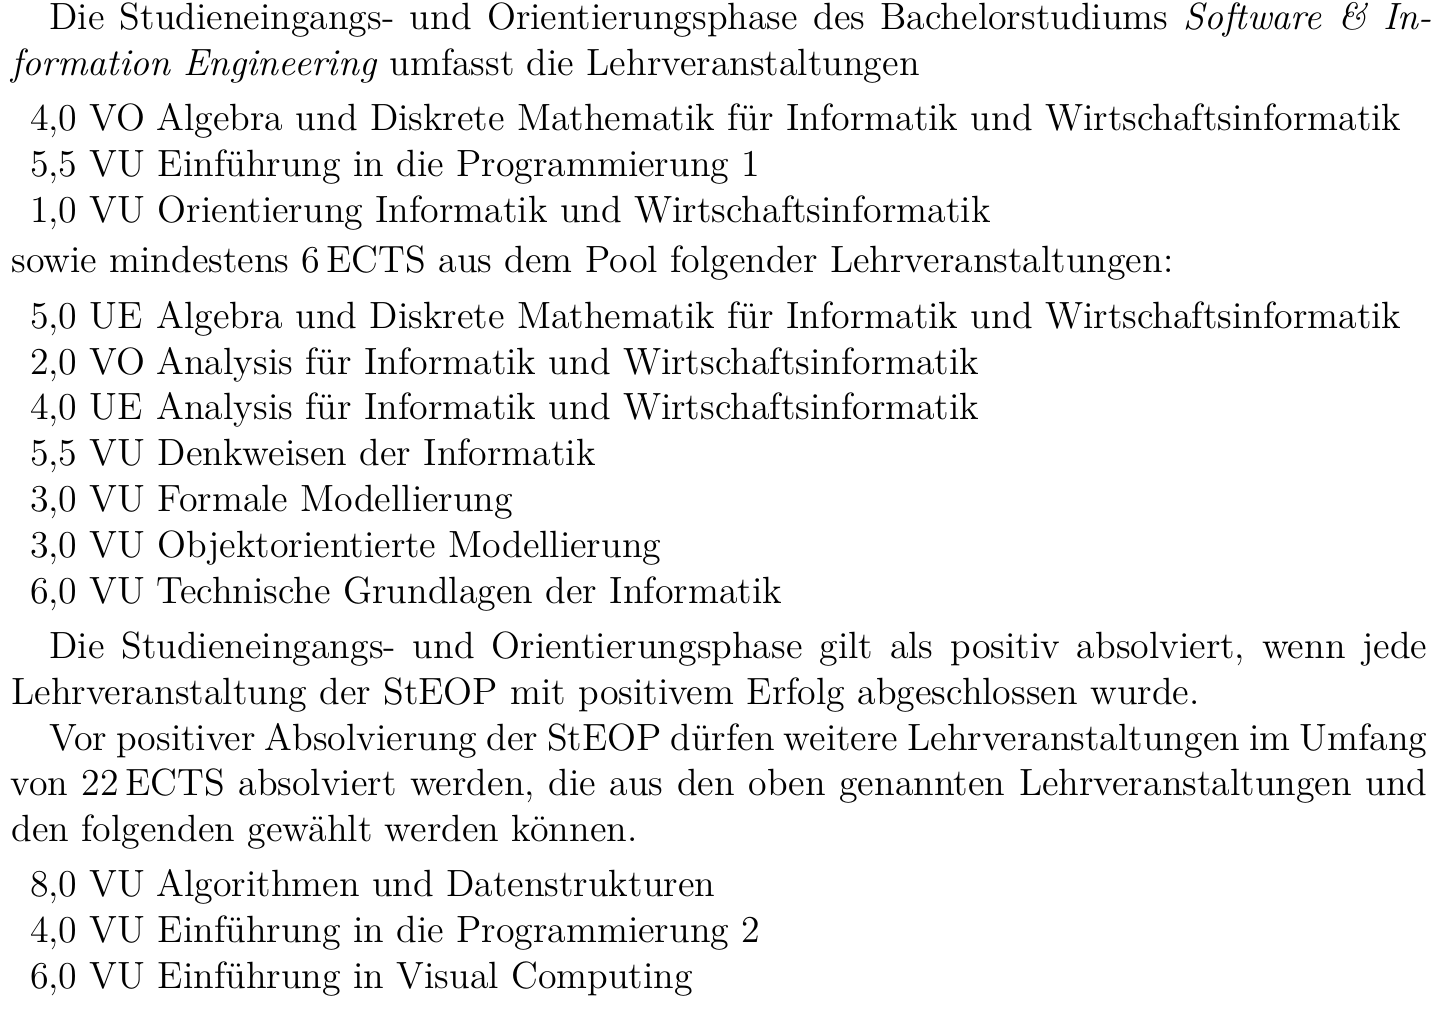
\includegraphics[width=1\textwidth]{steop.png}
    \end{figure}
    \tiny \textbf{Quelle:} Studienplan \textit{Bachelor Software \&
        Information Engineering} 2017W
\end{frame}

\section{LVA-Typen}
\begin{frame}{LVA-Typen}
    \begin{itemize}
    \item VO = Vorlesung.
          Leistungsnachweis: Prüfung.
    \item UE = Übung.
          z.B. Algebra: wöchentliche Termine.
          Leistungsnachweis: Kreuzerln, Tests, Tafelmeldungen.
    \item VU = Vorlesung mit Übung.
          Leistungsnachweis: Note darf nicht nur aus einer Prüfung stammen.
    \end{itemize}
\end{frame}

\section{Semesterempfehlung}
\begin{frame}{Semesterempfehlung}
    \begin{figure}[htp]
        \centering
        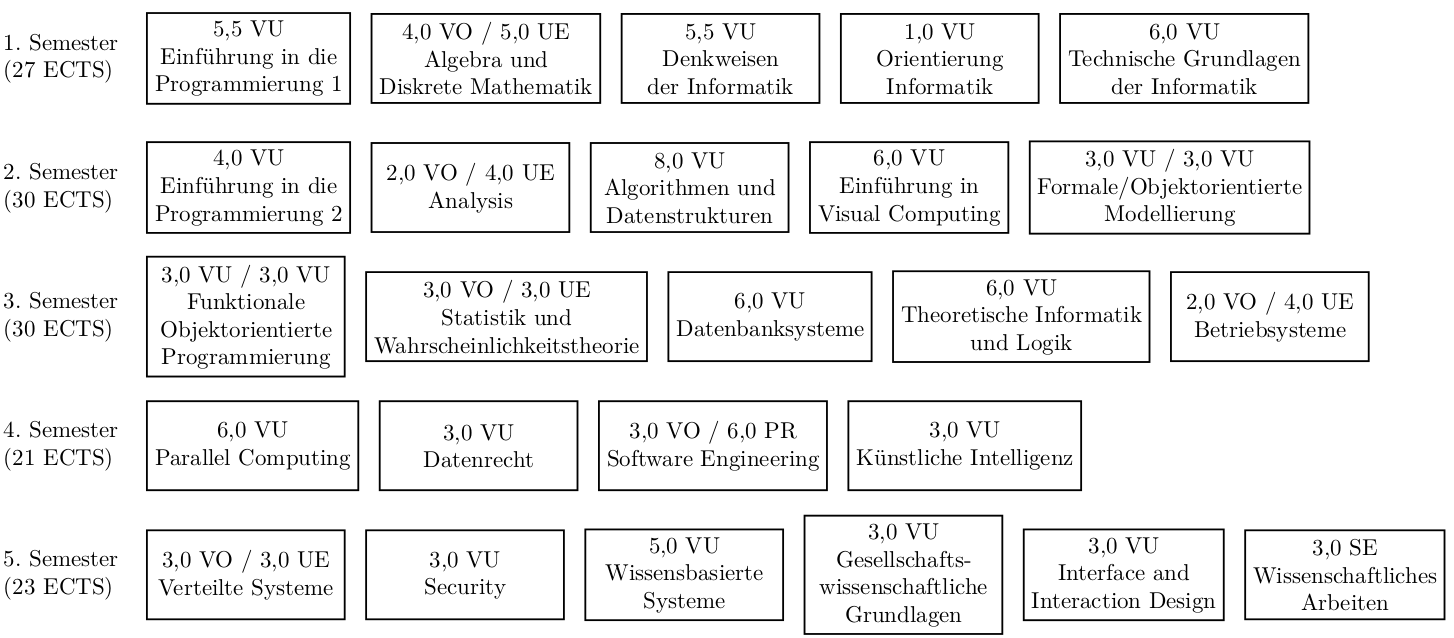
\includegraphics[width=1\textwidth]{semesterempfehlung.png}
    \end{figure}
    \tiny \textbf{Quelle:} Studienplan \textit{Bachelor Software \&
        Information Engineering} 2018W
\end{frame}

\subsection{Algebra und Diskrete Mathematik}
\begin{frame}{Algebra und Diskrete Mathematik}
    \begin{itemize}
        \item \textbf{VO:} nur Prüfungsanmeldung (6 Prüfungen pro Semester)
        \item \textbf{UE:} tatsächliche Termine und Beispiele auf eigener Website
        \item Freie Wahl des Prüfers (Gittenberger, Panholzer, Dorfer)
            \footnote{Haupttermin unbegrenzt viele Plätze, Nebentermine nur 80-120}
        \item Tipp: Panholzer $>$ Dorfer $>$ Gittenberger
            \begin{itemize}
                \item (Karigl leider schon in Pension)
            \end{itemize}
        \item \textbf{Kein Taschenrechner erlaubt!}\footnote{seit Juni 2016}
    \end{itemize}
\end{frame}

\begin{frame}{Erlaubte Formelsammlung}
    \begin{figure}[htp]
        \centering
        \subfloat[Alte Auflage]{
\includegraphics[width=0.35\textwidth]{formelsammlung.png}}
        \hfill
        \subfloat[13. Auflage von 2017]{
\includegraphics[width=0.35\textwidth]{formelsammlung2017.png}}
    \end{figure}
    \begin{itemize}
        \item ISBN: 978-3-209-10079-5
        \item Preis: 6{,}21 €; z.\,B. bei INTU.books oder Morawa
    \end{itemize}
\end{frame}

\subsection{LVAs}
\begin{frame}{LVAs}
    \begin{itemize}
        \item Denkweisen der Informatik VU
        \item Einführung in die Programmierung 1 VU
        \item Orientierung Informatik und Wirtschaftsinformatik VU
        \item Technische Grundlagen der Informatik VU
    \end{itemize}
\end{frame}

\section{Begriffsdefinitionen}

\begin{frame}{Begriffsdefinitionen}
    Es folgen einige Begriffe, die oft verwendet werden und nicht immer klar
    sind.
\end{frame}

\begin{frame}{Studienplan}
    \begin{itemize}
        \item Der Studienplan regelt das Studium und teilt es in mehrere
              \textit{Prüfungsfächer} auf.
        \item Ein \textit{Prüfungsfach} besteht aus \textit{Modulen}, diese
              bestehen aus \textit{Lehrveranstaltungen}.
        \item Eine \textit{Lehrveranstaltung (LVA)} ist z.\,B. eine
              \textit{Vorlesung (VO)}, \textit{Übung (UE)} oder
              \textit{Vorlesung mit Übung (VU)}.
    \end{itemize}
    Der aktuellste Studienplan ist unter
    \url{http://www.informatik.tuwien.ac.at/studium/angebot/studienplaene}
    zu finden.
\end{frame}

\begin{frame}{Beispiel für ein Prüfungsfach}
    Aus dem Bachelorstudium \textit{Software \& Information Engineering}: \\
    \begin{figure}[htp]
        \centering
        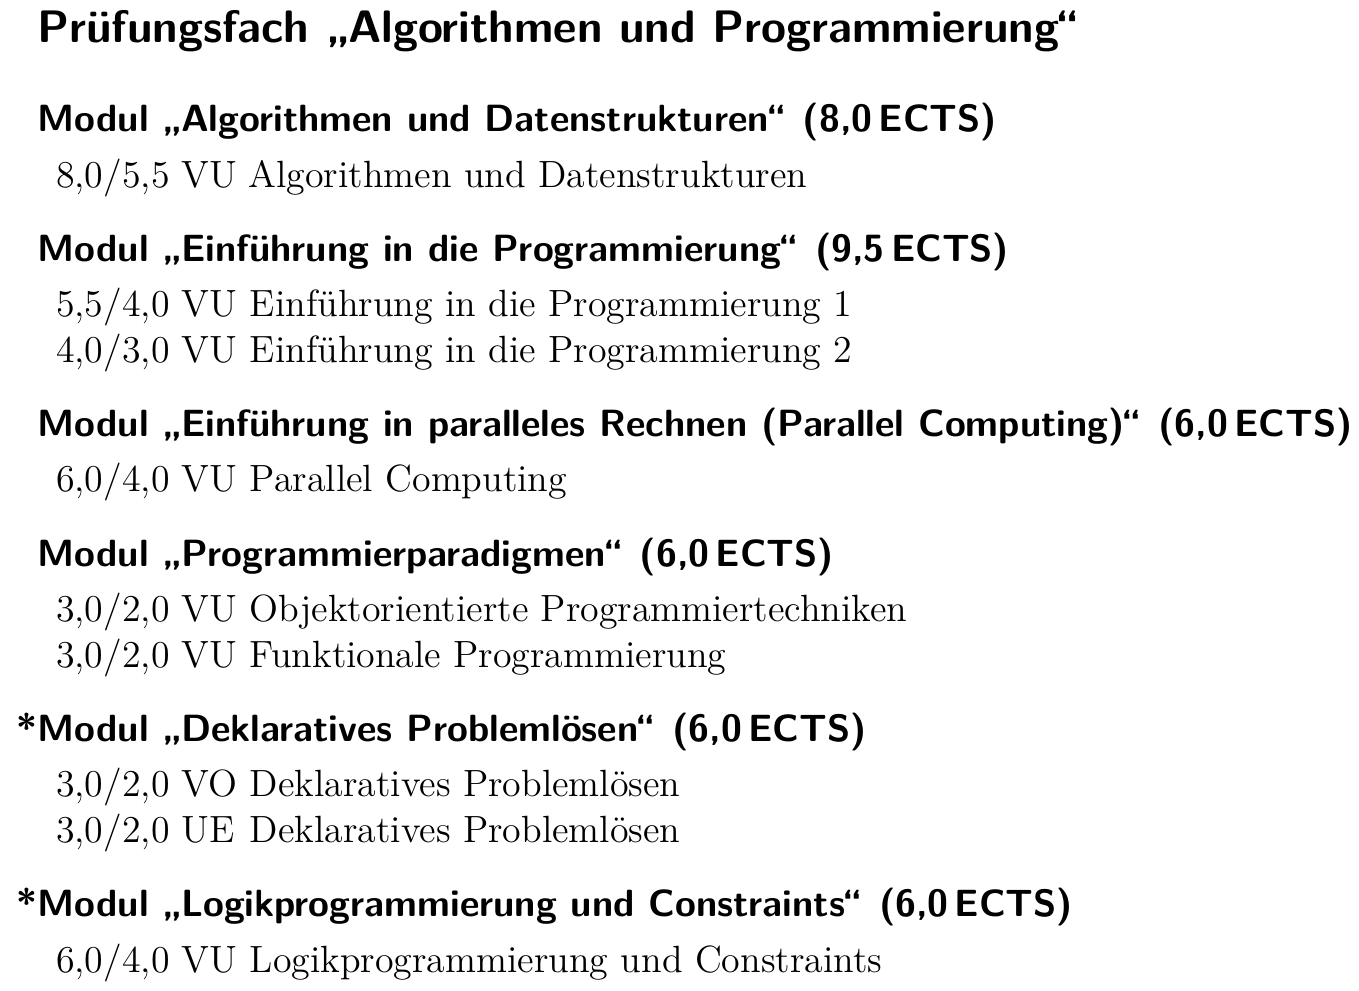
\includegraphics[width=0.8\textwidth]{pruefungsfach.png}
    \end{figure}
    \small Die mit Stern markierten Module sind \textit{Wahlmodule}, die anderen
          \textit{Pflichtmodule}.
\end{frame}

\begin{frame}{Pflichtmodul}
    \begin{itemize}
        \item Ein \textit{Pflichtmodul} ist ein Modul, das
              \textit{in jedem Fall} absolviert werden muss.
        \item Ein Pflichtmodul besteht daher aus \textit{Pflicht-LVAs}.
    \end{itemize}
\end{frame}

\begin{frame}{Wahlmodul}
    \begin{itemize}
        \item Ein \textit{Wahlmodul} ist ein Modul, das
              \textit{unter Umständen} absolviert werden muss.
        \item Ein Wahlmodul besteht daher aus \textit{Wahl-LVAs}.
        \item Studienplan gibt vor, \textit{wieviele ECTS} an Wahlmodulen
              absolviert werden müssen.
        \item \textbf{Beispiel:} In SE müssen min. 21 ECTS gewählt werden.
        \item \textbf{Wichtig:} Jedem Modul ist eine Anzahl an ECTS
              zugeordnet. Das Modul ist erst vollständig absolviert, wenn
              diese Anzahl erreicht wird.
        \item Wahl-LVAs werden auch als \textit{Wahlfächer} bezeichnet.
    \end{itemize}
\end{frame}

\begin{frame}{Wahlmodul (2)}
    Bei manchen Wahlmodulen wie z.\,B. \textit{Security} kann auch
    \textit{innerhalb} des Moduls gewählt werden!
    \begin{figure}[htp]
        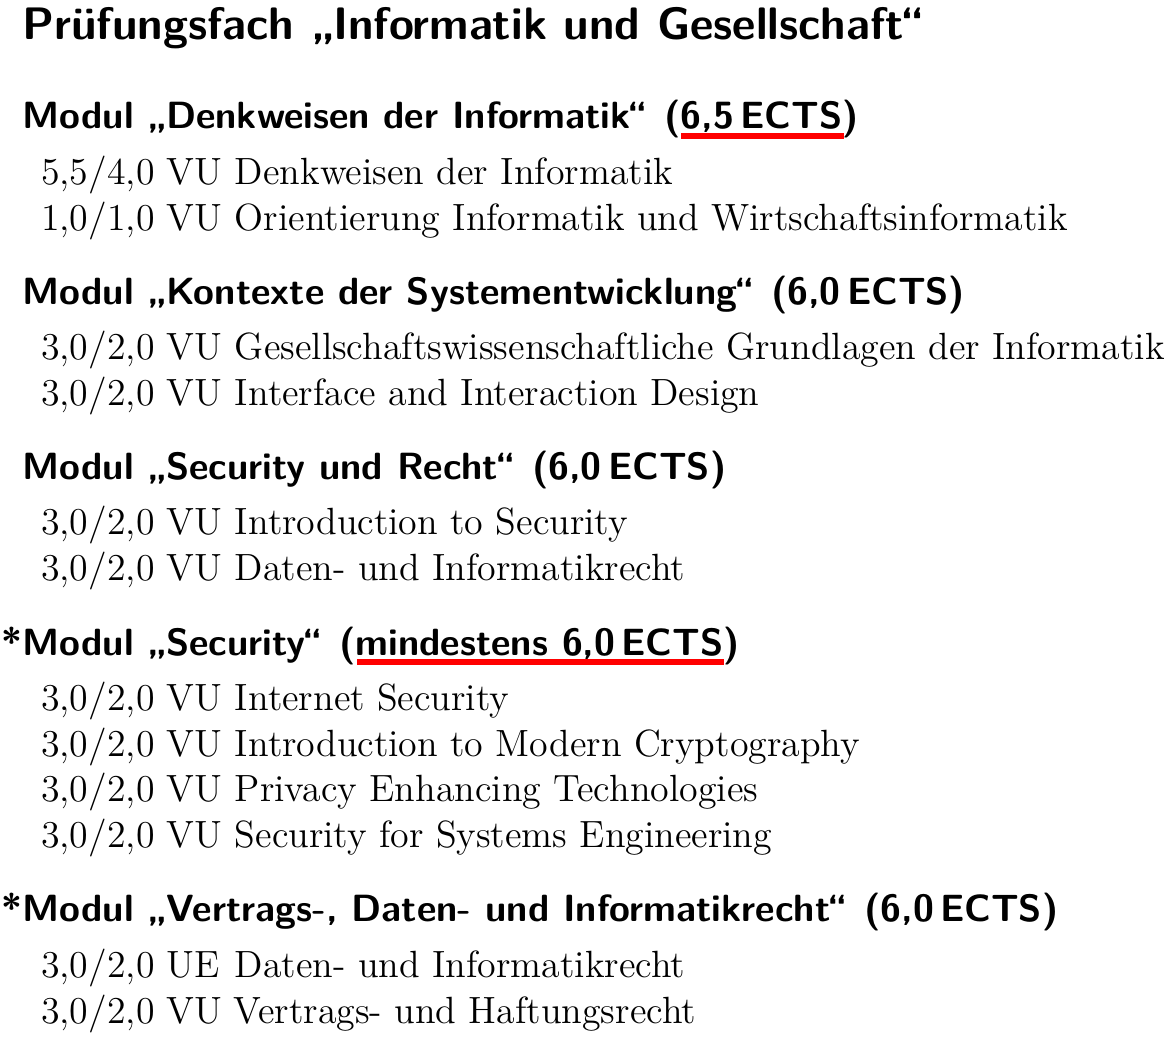
\includegraphics[width=0.7\textwidth]{pruefungsfach2.png}
    \end{figure}
\end{frame}

\begin{frame}{Wahlmodul (3)}
    Nehmt euren Studienplan zur Hand, damit ihr wisst, \ldots
    \begin{itemize}
        \item \ldots{} wie viele Wahl-LVAs ihr absolvieren müsst.
        \item \ldots{} welche Wahl-LVAs es \textit{in eurem Studium} überhaupt
            gibt.
    \end{itemize}
\end{frame}

\begin{frame}{Spezialfall: Freie Wahlfächer}
    \begin{figure}[htp]
        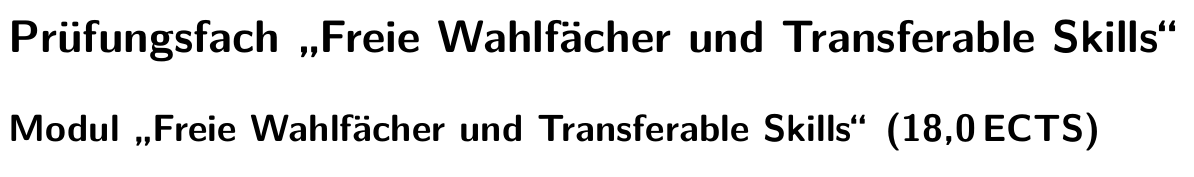
\includegraphics[width=1.0\textwidth]{pruefungsfach3.png}
    \end{figure}
    \begin{itemize}
        \item Einen kleinen Teil eures Studiums könnt ihr quasi völlig frei
              aussuchen und auch auf anderen Unis absolvieren!
        \item \textbf{Beispiel:} In Software \& Information Eng. sind das 12 ECTS.
        \item Diese LVAs werden auch als \textit{Freifächer} oder
              \textit{Freie Wahlfächer} bezeichnet.
        \item \textbf{Wichtig:} STEOP ist hier keine Voraussetzung!
    \end{itemize}
\end{frame}

\begin{frame}{Spezialfall: Transferable Skills (TFS)}
    \begin{figure}[htp]
        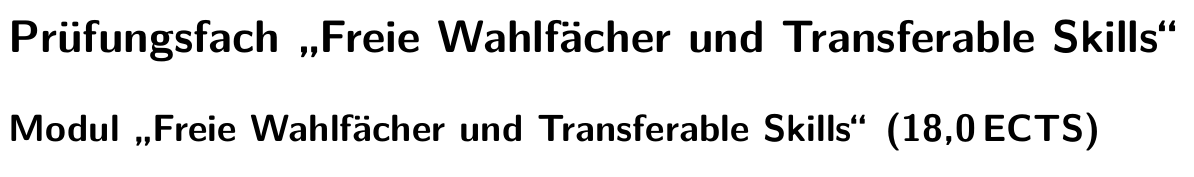
\includegraphics[width=1.0\textwidth]{pruefungsfach3.png}
    \end{figure}
    \begin{itemize}
        \item Ein kleiner Teil eures Studiums soll euch in allgemeinen
              Bereichen wie Rhetorik, Didaktik, o.\,ä. stärken.
        \item \textbf{Beispiel:} In Software \& Information Eng. sind das 6 ECTS.
        \item Diese LVAs werden auch als \textit{Soft Skills} bezeichnet.
        \item Im TISS gibt es eine eigenen \textit{Transferable
              Skills}-Katalog (zu finden unter \textit{Studienangebot})
        \item \textbf{Wichtig:} STEOP ist hier keine Voraussetzung!
    \end{itemize}
\end{frame}

\begin{frame}{Wo finde ich den Transferable Skills (TFS)-Katalog?}
    \begin{figure}[htp]
        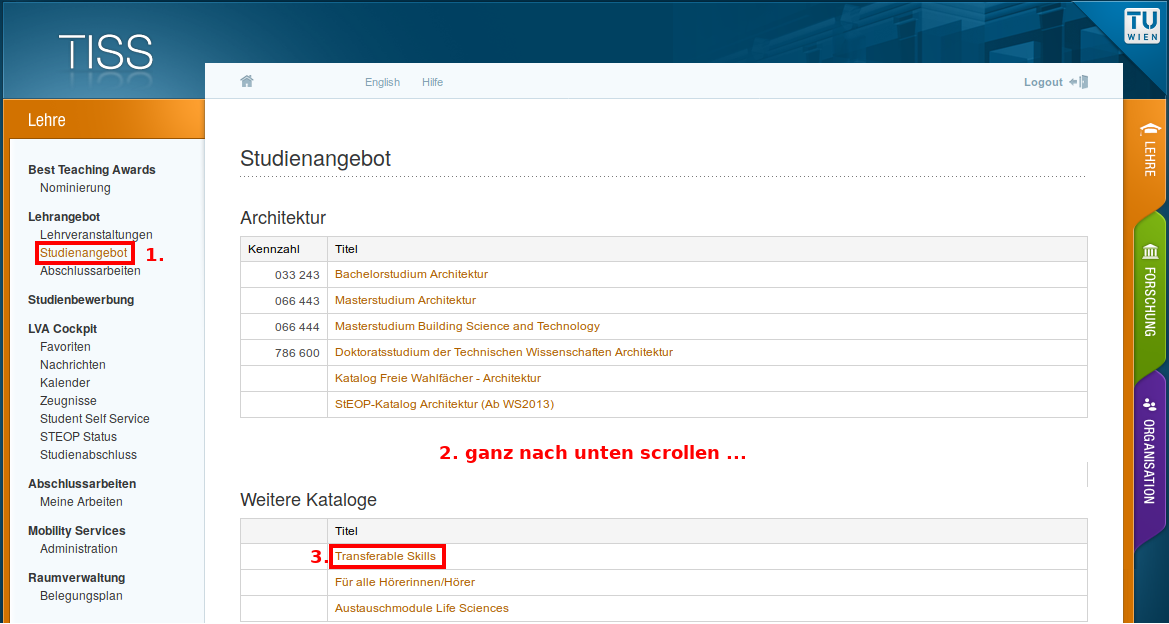
\includegraphics[width=1.0\textwidth]{tiss_tfs.png}
    \end{figure}
     \url{https://tiss.tuwien.ac.at/curriculum/public/curriculum.xhtml?key=57214}
\end{frame}

\section{TISS -- ganz kurz}
\begin{frame}{TISS -- ganz kurz}
    \begin{itemize}
        \item Favoriten
        \item LVA-Kataloge
        \item Studienplan
        \item Zeugnisse \& Bestätigungen
    \end{itemize}
\end{frame}

\section{Weitere Hilfestellungen}
\begin{frame}{Wo finde ich \ldots}
    \begin{itemize}
        \item \textit{\ldots{} diese Folien zum Download?} \\
              $\Rightarrow$ \url{https://bit.ly/2UvQINa}
        \item \textit{\ldots{} Materialien zu LVAs wie alte Testangaben?} \\
              $\Rightarrow$ VoWi -- Das Vorlesungswiki enthält Materialien und
              Erfahrungsberichte zu LVAs: \url{vowi.fsinf.at}
        \item \textit{\ldots{} andere Informatik-Studierende, mit denen ich
              chatten kann?} \\
              $\Rightarrow$ Mattermost-Chat der FSINF: \url{mattermost.fsinf.at}
        \item \textit{\ldots{} jemanden im Real Life?} \\
              $\Rightarrow$ FSINF (Treitlstraße 3, Hochparterre)
    \end{itemize}
\end{frame}

\section*{Abschluss}
\begin{frame}{Fragen}
    Eure Fragen sind jetzt gefragt!\\
    \vspace{2cm}
    Diese Folien zum Download: \url{https://bit.ly/2UvQINa}
\end{frame}

\begin{frame}{\ldots und weiter?}
    \begin{itemize}
        \item Beratung und Chat der FSINF: \url{https://mm.fsinf.at}
        \item Beratung auch via \url{beratung@fsinf.at}
        \item Leitfaden für Erstsemestrige: \url{https://fsinf.at/basics}
    \end{itemize}

    \vspace{2cm}
    Diese Folien zum Download: \url{https://bit.ly/2UvQINa}
\end{frame}

\end{document}
